\documentclass[border=10pt]{standalone}

%Drawing
\usepackage{tikz}
\usetikzlibrary{intersections}
\usetikzlibrary{calc}


\newcommand{\drawRectangle}[2]{
   	\draw[fill=blue, opacity=0.2] ($(#1,#2) - (0.5,0.5)$) rectangle ($(#1,#2) + (0.5,0.5)$) ;   
}

\begin{document}
	
	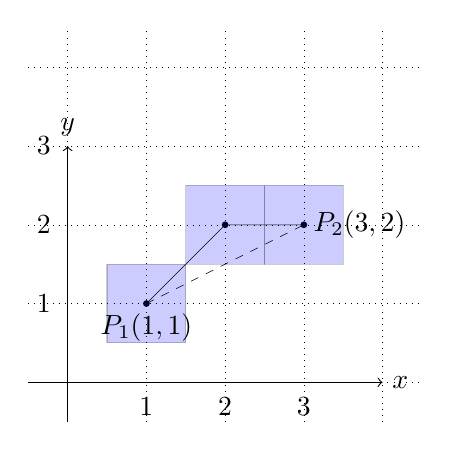
\begin{tikzpicture}
%%%%%%%%%%%%%%%%%%	

%Grid
	\draw[very thin, dotted] (-0.5,-0.5) grid (4.5,4.5);
	\foreach \i in {1,...,3}
	{
		\node at (\i,-2ex) {\i};	
		\node at (-2ex,\i) {\i};				
	}

%Draw axes
    \draw[->] (-0.5, 0) -- (4, 0) node[right] {$x$};
    \draw[->] (0, -0.5) -- (0, 3) node[above] {$y$};
    
    
% Plot points
    \filldraw[black] (1, 1) circle (1pt) ;
	\filldraw[black] (2, 2) circle (1pt) ;
    \filldraw[black] (3, 2) circle (1pt); 

%	\fill[blue, opacity=0.2] (1,1) rectangle (2,2) ; 
\drawRectangle{1}{1}   
\drawRectangle{2}{2}
\drawRectangle{3}{2}   
% Connect points with a line
    \draw[very thin] (1, 1) -- (2, 2) -- (3, 2);
    \draw[dashed, very thin] (1, 1) -- (3, 2);

\node[below] at (1,1) {$P_1(1,1)$};
    \node[right] at (3,2) {$P_2(3,2)$};
    
\end{tikzpicture}

\end{document}



